\documentclass%
%[handout]
{beamer}
% % % % % % % %
% % % % % % % %
% % % % % % % %
%IMPORTANT
%compiles with 
%pdflatex -shell-escape 
%IMPORTANT
% % % % % % % %
% % % % % % % %
% % % % % % % %
\mode<presentation>
{
\useinnertheme{rounded}
\useoutertheme{infolines}
\usecolortheme{orchid}
\usecolortheme{whale}
}

\usepackage[english]{babel}
\usepackage[latin1]{inputenc}
\usepackage{times}
\usepackage[T1]{fontenc}
\usepackage{../example-templates}
\usepackage{auto-pst-pdf}
\usepackage{pst-plot}

% Or whatever. Note that the encoding and the font should match. If T1
% does not look nice, try deleting the line with the fontenc.

\graphicspath{{../../modules/}}

\newtheoremstyle{partialproof}{3pt}{3pt}{}{}{}{.}{.5em}{}
\theoremstyle{partialproof} \newtheorem{partialproof}[theorem]{Proof.}
%\DeclareMathOperator{\diff}{d}
\newcommand{\diff}{\text{d}}
\setbeamertemplate{navigation symbols}{}

\includeonlylecture{1}

\newcommand{\lect}[3]{
  \date{#1}
  \lecture[#1]{#2}{#3}
}

\setbeamertemplate{footline}
{
  \leavevmode%
  \hbox{%
  \begin{beamercolorbox}[wd=.333333\paperwidth,ht=2.25ex,dp=1ex,center]{author in head/foot}%
    \usebeamerfont{author in head/foot}\insertshortauthor
  \end{beamercolorbox}%
  \begin{beamercolorbox}[wd=.333333\paperwidth,ht=2.25ex,dp=1ex,center]{title in head/foot}%
    \usebeamerfont{title in head/foot}\insertshorttitle
  \end{beamercolorbox}%
  \begin{beamercolorbox}[wd=.333333\paperwidth,ht=2.25ex,dp=1ex,center]{date in head/foot}%
    \usebeamerfont{date in head/foot}\insertshortdate{}
  \end{beamercolorbox}}%
  \vskip0pt%
}

% If you have a file called "university-logo-filename.xxx", where xxx
% is a graphic format that can be processed by latex or pdflatex,
% resp., then you can add a logo as follows:

%\pgfdeclareimage[height=0.8cm]{logo}{bluelogo}
%\logo{\pgfuseimage{logo}}

\begin{document}
\newcommand{\psHollowDot}[2]{
\pscircle*[fillcolor=white, linecolor=red](#1, #2){0.07}
\pscircle*[fillcolor=white, linecolor=white](#1, #2){0.04}
}
\newcommand{\psFullDot}[2]{
\pscircle*[fillcolor=white, linecolor=red](#1, #2){0.07}
}
\newcommand{\psLabelXOne}{\psline(1, -0.1)(1,0.1) \rput[t](1, -0.2 ) {\footnotesize $1$} }
\newcommand{\psLabelYOne}{\psline(-0.1, 1)(0.1, 1) \rput[r](-0.2, 1 ) {\footnotesize $1$} }

\AtBeginLecture{%

\title[\insertlecture]{FreeCalc}
\subtitle{\insertlecture}
\author[FreeCalc]{}
\institute[UMass Boston]{University of Massachusetts Boston}
\date{\insertshortlecture}
\begin{frame}
  \titlepage
\end{frame}
}%

% begin lecture
\lect{\today}{Sample}{1}
% begin module infinite-limit-at-infinity-ex11
\begin{frame}
\begin{example}%[Example 11, p. 237]
Find the limits as $x\to \infty$ and $x\to -\infty$ of $y = (x-2)^4(x+1)^3(x-1)$.
%\begin{columns}[c]
%\column{.5\textwidth}
\begin{center}
\ \only<handout:0| -8>{%
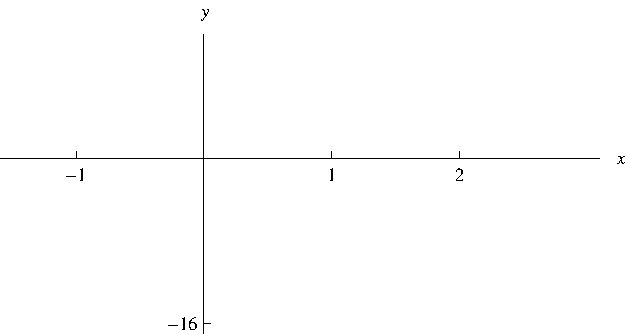
\includegraphics[width=7cm]{curve-sketching/pictures/04-04-ex11a.pdf}%
}%
\only<handout:0| 9-15>{%
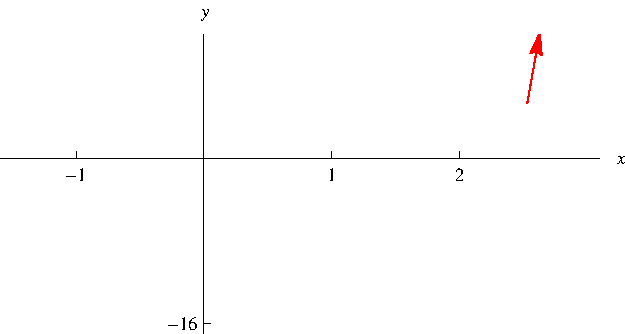
\includegraphics[width=7cm]{curve-sketching/pictures/04-04-ex11b.pdf}%
}%
\only<handout:0| 16>{%
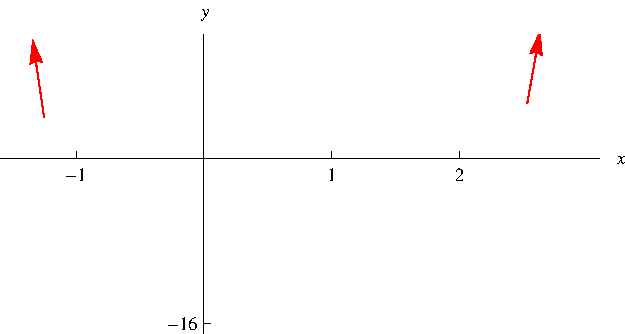
\includegraphics[width=7cm]{curve-sketching/pictures/04-04-ex11c.pdf}%
}%
\only<17->{%
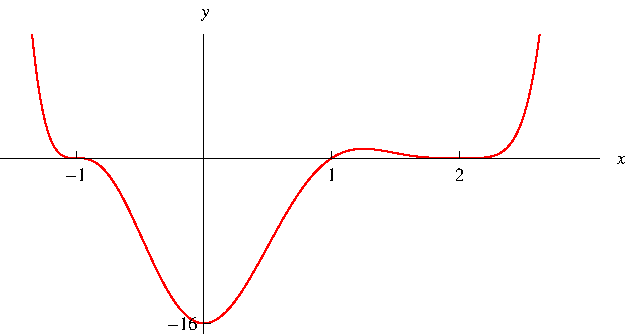
\includegraphics[width=7cm]{curve-sketching/pictures/04-04-ex11d.pdf}%
}%
\end{center}
\uncover<2->{%
\abovedisplayskip=0pt
\belowdisplayskip=0pt
\[
\begin{array}{c@{}c@{}c@{}ccr}
\displaystyle \lim_{x\to \infty}&%
\alert<handout:0| 3-4>{(x-2)^4}&%
\alert<handout:0| 5-6>{(x+1)^3}&%
\alert<handout:0| 7-8>{(x-1)}&%
 = &%
\uncover<9->{\alert<handout:0| 9>{\infty}}%
\\%
&%
\uncover<4->{\alert<handout:0| 4,9>{+}}&%
\uncover<6->{\alert<handout:0| 6,9>{+}}&%
\uncover<8->{\alert<handout:0| 8,9>{+}}&%
&\\%
&&&&&\\%
\displaystyle \lim_{x\to -\infty}&%
\alert<handout:0| 10-11>{(x-2)^4}&%
\alert<handout:0| 12-13>{(x+1)^3}&%
\alert<handout:0| 14-15>{(x-1)}&%
 = &%
\uncover<16->{\alert<handout:0| 16>{\infty}}%
\\%
&%
\uncover<11->{\alert<handout:0| 11,16>{+}}&%
\uncover<13->{\alert<handout:0| 13,16>{-}}&%
\uncover<15->{\alert<handout:0| 15,16>{-}}&%
&%
\end{array}
\]
}%
\vspace{-.1in}
%\end{columns}
\end{example}
\end{frame}
% end module infinite-limit-at-infinity-ex11

% end lecture

\end{document}
